\documentclass[paper=128mm:96mm, fontsize=9pt, pagesize]{scrartcl}

\linespread{1.12}

\usepackage{soul}
\usepackage[default]{opensans}
\linespread{1.05}
\usepackage{microtype}

\setlength{\parskip}{0pt}

\usepackage[hang, small,labelfont=bf,up,textfont=it,up]{caption}
\usepackage[hidelinks, colorlinks=true]{hyperref}
\usepackage{booktabs, float, paralist, abstract, titling, enumitem, graphicx}
\usepackage[compact]{titlesec}
\usepackage[usenames,dvipsnames,svgnames,table]{xcolor}
\usepackage[flushmargin,hang,multiple]{footmisc}
\interfootnotelinepenalty=10000

\usepackage[includeheadfoot, top=4mm, bottom=4mm, left=6mm, right=6mm, headsep=6.5mm, footskip=8.5mm]{geometry}

\renewcommand{\abstractnamefont}{\normalfont\large\sffamily}
\renewcommand{\abstracttextfont}{\normalfont\itshape}

\titleformat*{\section}{\Large\sffamily}
\titleformat*{\subsection}{\large\sffamily}
\titleformat*{\subsubsection}{\itshape\sffamily}
\titleformat*{\paragraph}{\large\bfseries\sffamily}
\titleformat*{\subparagraph}{\large\bfseries\sffamily}
\titlespacing*{\section}
{0pt}{0pt}{0pt}
\titlespacing*{\subsection}
{0pt}{0pt}{0pt}

\setlist[description]{format=\normalfont\itshape}

\renewcommand{\maketitle}{\noindent\rule{\linewidth}{1pt}\Huge \vspace{1em} \newline
\sffamily \scshape \thetitle \\
\normalfont \sffamily  \theauthor \\
\thedate
\newline\noindent\rule{\linewidth}{1pt}
\normalfont
\normalsize}

\pagestyle{empty}


\title{Let's Talk About Boxes}
\author{
\normalsize
{Calem Bendell} \\
Hyvedev, McGill University \\
\href{mailto:calem.bendell@mail.mcgill.ca}{calem.bendell@mail.mcgill.ca}
}
\date{}

\begin{document}

\maketitle

\clearpage

\so{I LOVE BOXES}

a lot.
so now we've gotten that out of the way, let's move on to why I love boxes, and why you should too.

\clearpage

\section{this is a stainless steel cube.}
\subsection{the cube is arguably the 2nd most beautiful geometric concept.  it is the most basic 3 dimensional equilateral shape in existence.}
\begin{figure}
	\centering
	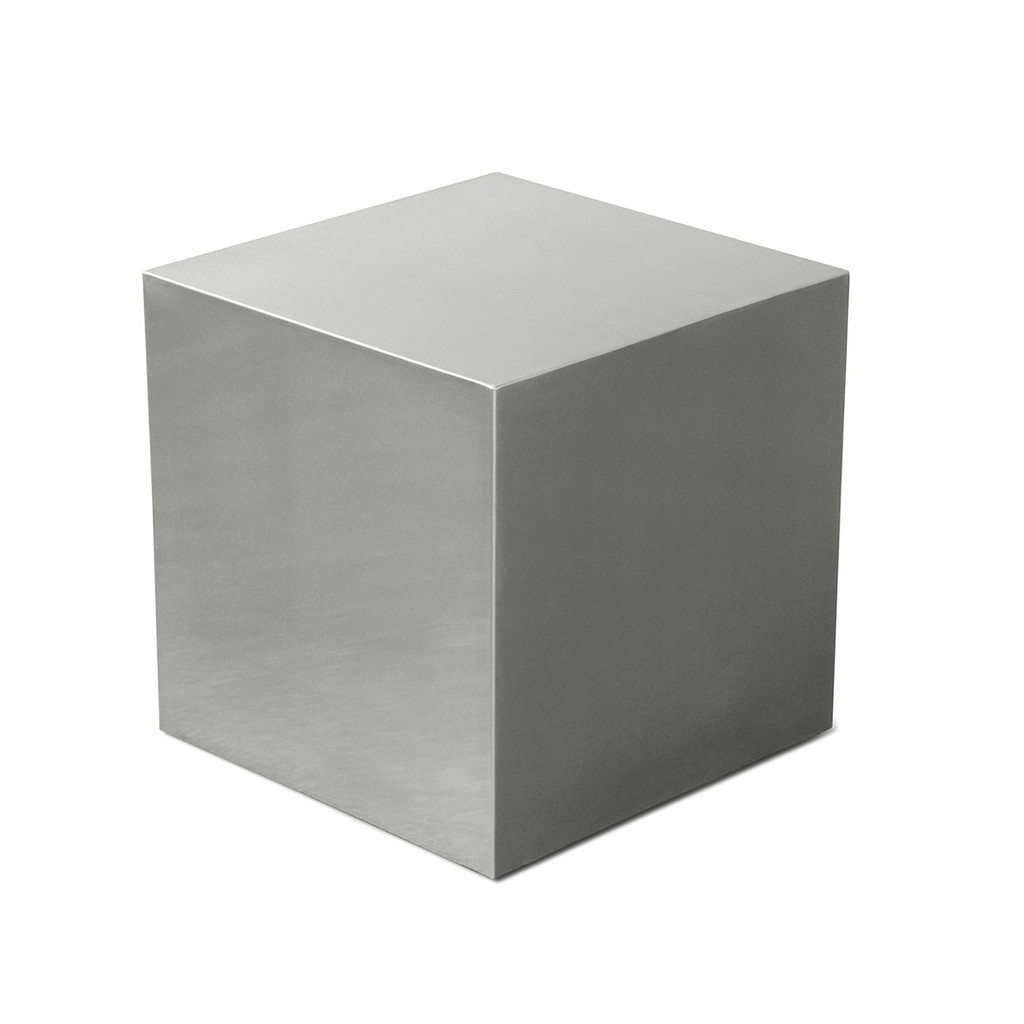
\includegraphics[height=.5\textheight]{gfx/cube1.jpg}
\end{figure}

\clearpage

\section{this is a cube made of cubes.}
\subsection{cubes can be easily stacked and arranged in any way.  same goes for boxes of the same shape.}
\begin{figure}
	\centering
	
\includegraphics[height=.5\textheight]{gfx/modularcube.jpg}
\end{figure}

\clearpage

\section{this is a borg cube.}
\subsection{even the borg love the cube.  the first officially publicized federation contact with a borg cube will be in 2365, an encounter with a single cube in system j-25.  the borg know and love the cube.}
\begin{figure}
	\centering
	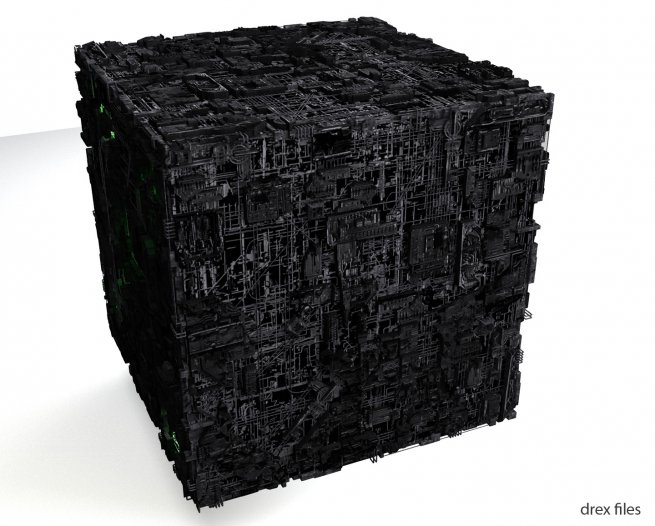
\includegraphics[height=.5\textheight]{gfx/borgbox.jpg}
\end{figure}

\clearpage

\section{this is a rectangle.}
\subsection{let's move on to arguably the most beautiful geometric shape.  this shape isn't equilateral, but a special case of it has a shitton of beautiful properties.}
\begin{figure}
	\centering
	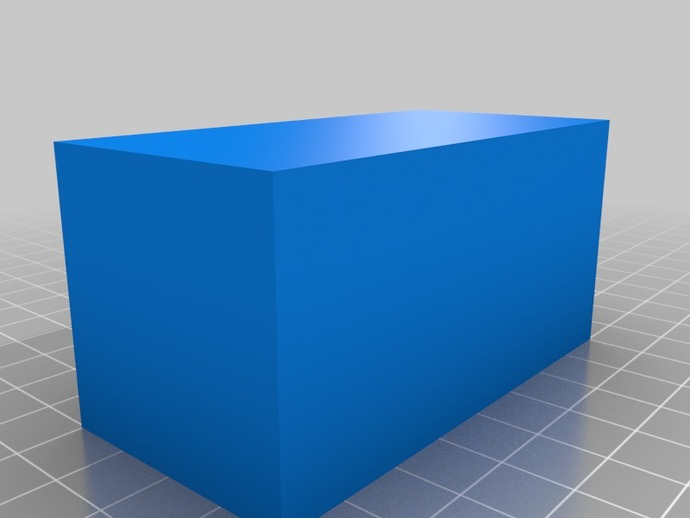
\includegraphics[height=.5\textheight]{gfx/rectangle1.jpg}
\end{figure}

\clearpage

\section{behold the harmonic chamber.}
\subsection{this golden ratio rectangle is used by sound designers all around the world.  it is the essence of concert halls for its acoustic properties}
\begin{figure}
	\centering
	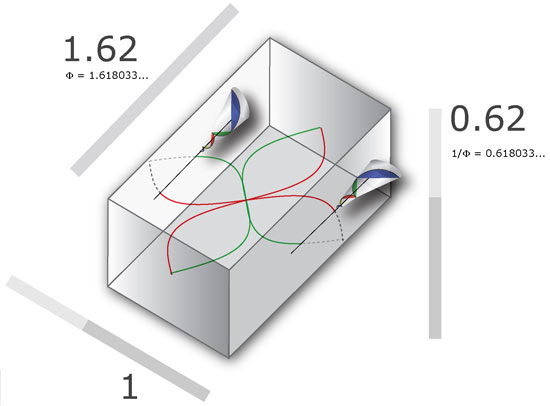
\includegraphics[height=.5\textheight]{gfx/harmonic_chamber.jpg}
\end{figure}

\clearpage

\section{this is part of the reason why harmonic chambers work.}
\subsection{it's a harmonic formation.  it's pretty sick, and you should look it up!  but it's out of the scope of this discussion.  basically sound will resonate and carry nicely in this shape.  as i understand it, this counts for most of fluid dynamics and general wave dynamics.}
\begin{figure}
	\centering
	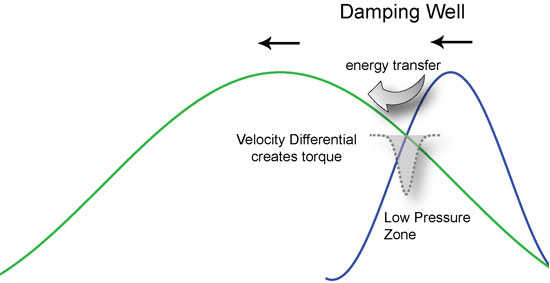
\includegraphics[height=.5\textheight]{gfx/harmonics_dampingW.jpg}
\end{figure}

\clearpage

\section{Dr. Edith Farnsworth House}
\subsection{This is an icon in modern architecture.  It follows the golden ratio and several other mathematical features to make itself an incredibly pleasing shape for a rectangle.}
\begin{figure}
	\centering
	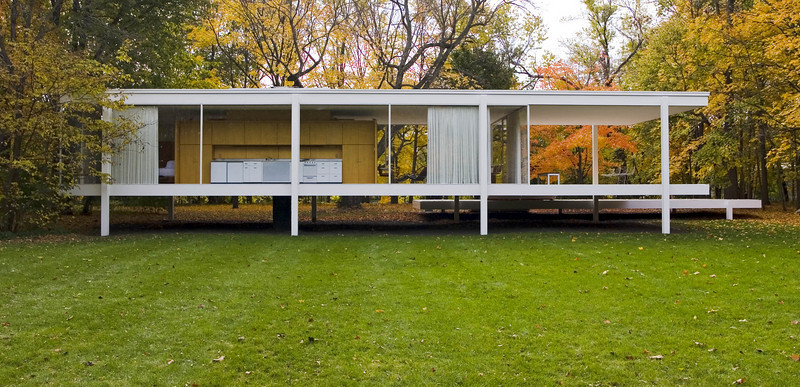
\includegraphics[height=.5\textheight]{gfx/41735665_psh2G-L-2.jpg}
\end{figure}

\clearpage

\section{our house?}
\subsection{how does this all relate to our house?  the above is pretty damn beautiful}
\begin{figure}
	\centering
	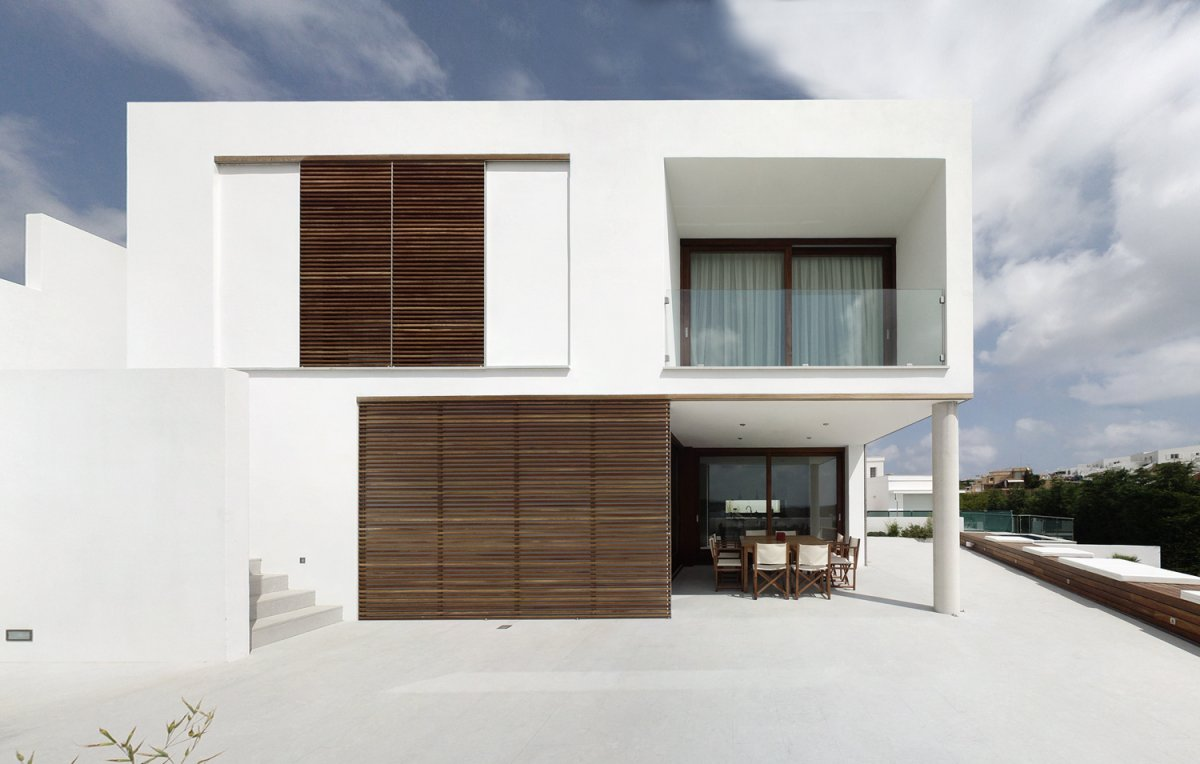
\includegraphics[height=.5\textheight]{gfx/modern-minimalist-square-house-menorca-sun-shades-for-the-windows-ideas.jpg}
\end{figure}

\clearpage

\section{let's get a little more serious}

the current house designs are great, but they're a little complicated.
we want to score maximum points with a low price, right?
low price and minimal assembly.
minimalism in general would work in our favour.

what if the house was one massive room excepting the bathroom (only one bathroom...) and the mechanical room and the bedroom?
instead of a full second floor, two lofts that face each other, maybe one of them closed as a bedroom but with no particular ceiling.
what if that massive room was built according to the golden ratio, maximising its beauty and acoustics?

\clearpage

\section{advantages}

circulation is much easier.
automation is easier.
taking advantage of natural lighting is as simple as putting in a lot of windows.
we'll be saving a lot of money with the simple construction.

\section{fluid dynamics (weak point... maybe ignore it, but i think it's wicked)}

oh yeah, did i mention the golden ratio is important in fluid dynamics?
the golden ratio is also considered in the construction of modern wind tunnels.
i don't really understand the papers i read particularly well, but basically, we might be able to prove that air circulation can be improved by taking advantage of the golden ratio to create certain currents.
that is, so far as i know, innovative, effective, subtle, and beautiful.
i might be wrong on that, since i didn't understand the literature particularly well, but it may be something worth exploring.

\clearpage

\section{interior design}

you give the interior design team an open canvas.
\begin{figure}
	\centering
	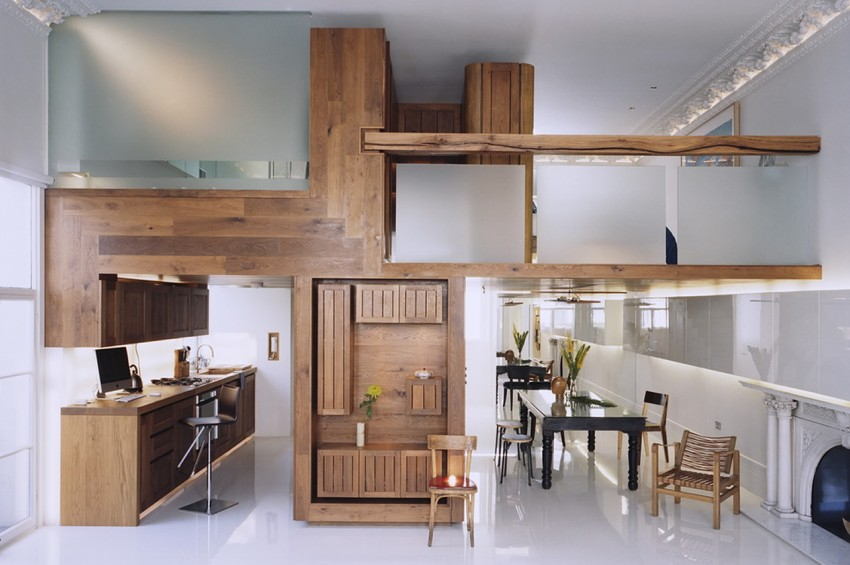
\includegraphics[height=.6\textheight]{gfx/humblehomespace.jpg}
\end{figure}

\clearpage

\section{automation}

every aspect of the automation team's job is simplified.
we need much less equipment, don't need to worry about interference, don't need to worry too much about wiring.

\clearpage

\section{structure}

it's a rectangle with some cool loft and interior structures.
'nuff said, i think.

\clearpage

\section{envelope}

with the freedom to spend all of their time worrying about insulation and cool window dynamics, the envelope team is free to innovate by introducing ideals such as wind tunnels in the walls, which can be introduced due to the simplistic design of the structure.

\clearpage

\section{hvac}

i mentioned the fluid dynamics above.
let's explore that!
and you have an open space to worry about, which should dramatically simplify hvac.

\clearpage

\section{architecture}

architecture has significantly less to worry about regarding the shell of the house and can focus entirely on the interior and styling of the front and back of the house, the parts that are exposed.

\clearpage

\section{and so on}

i don't think i really need to keep going here.

so what the final design could look like really depends on windows and skylights.
if we invest in windows that tint and untint by electric shock, we have a lot of options in terms of adaptive cooling, privacy, and openness.
we can invest in the least flexible, most sustainable, most durable insulating materials.

everything becomes simpler.
simpler is good.

there are soooo many reasons to make the house a simple rectangle.

we probably barely know all the advantages that come with this geometric reasoning.
we'll sure as hell have a lot to discuss with the mathematicians. 

\clearpage

\so{ROCK ON! AND CONSIDER IT}

\end{document}